\PassOptionsToPackage{dvipsnames,svgnames,x11names}{xcolor}
\documentclass[tikz,border=8pt]{standalone}
\usetikzlibrary{arrows.meta,positioning,calc,shapes,shadows,decorations.pathmorphing,shapes.geometric,backgrounds,decorations.markings,decorations.pathreplacing,decorations.text,fit,shapes.misc,shapes.arrows,matrix,bending,3d,chains,intersections,shapes.symbols,svg.path,shapes.multipart,snakes,shapes.callouts,angles,quotes}
\providecolor{gold}{RGB}{212,175,55}
\providecolor{silver}{RGB}{192,192,192}
\providecolor{bronze}{RGB}{205,127,50}
\providecolor{darkblue}{RGB}{0,0,139}
\providecolor{lightblue}{RGB}{173,216,230}
\providecolor{darkgreen}{RGB}{0,100,0}
\providecolor{lightgreen}{RGB}{144,238,144}
\providecolor{darkred}{RGB}{139,0,0}
\providecolor{navy}{RGB}{0,0,128}
\providecolor{skyblue}{RGB}{135,206,235}
\providecolor{beige}{RGB}{245,245,220}
\providecolor{cream}{RGB}{255,253,208}
\usepackage{amsmath}
\usepackage{amssymb}
\usepackage{fontawesome5}
\usetikzlibrary{fadings,shadows.blur,patterns,patterns.meta}

% --- DEFINE CUSTOM COLORS ---
\definecolor{accentblue}{RGB}{41, 128, 185}
\definecolor{accentgreen}{RGB}{39, 174, 96}
\definecolor{accentorange}{RGB}{230, 126, 34}
\definecolor{textdark}{RGB}{44, 62, 80}
\definecolor{codebg}{RGB}{40, 44, 52}
\definecolor{codetext}{RGB}{171, 178, 191}

\begin{document}
\begin{tikzpicture}

% 1. BACKGROUND (Pure White Expanded Canvas with Safety Bounds)
\fill[white] (-0.5, -3.0) rectangle (21.0414,25.1601);

% 2. TITLE & INTENT (Zero-Overlap Header)
\node[font=\Huge\bfseries\color{textdark}, anchor=center] at (10.0414,23.6601) {Resolution Switching};
\node[font=\Large\color{textdark!80}, anchor=center, align=center, text width=16cm] at (10,21.4698) {Intent: Deliver the \textbf{identical image} composition, optimized for the screen's dimensions \\ and pixel density. The primary goal is \textbf{performance} and bandwidth savings.};

% 3. REUSABLE REALISTIC LANDSCAPE MACRO
\newcommand{\drawLandscape}[3]{
    % #1 = x, #2 = y, #3 = scale
    \begin{scope}[shift={(#1, #2)}, scale=#3]
        \begin{scope}
            \clip (-2, -1) rectangle (2, 1);

            % Dynamic Sky Gradient
            \shade[top color=MidnightBlue!90!NavyBlue, bottom color=Cyan!35] (-2, -1) rectangle (2, 1);

            % Realistic Sun with Radial Glow
            \shade[inner color=yellow!90!orange, outer color=Cyan!35, opacity=0.85] (1.1, 0.45) circle (0.45);
            \fill[yellow!95!white] (1.1, 0.45) circle (0.18);

            % Distant Mountain Range Profile
            \shade[top color=SlateGray!70!RoyalBlue, bottom color=MidnightBlue!80]
                (-2, -0.4) -- (-1.5, 0.2) -- (-0.8, -0.2) -- (-0.2, 0.4) -- (0.5, -0.2) -- (1.3, 0.25) -- (2, -0.3) -- (2, -1) -- (-2, -1) -- cycle;

            % Main Left Mountain with Shading & Snowcap
            \shade[left color=gray!80, right color=black!65] (-1.8, -0.5) -- (-0.85, 0.65) -- (0.1, -0.5) -- cycle;
            \fill[white, opacity=0.95] (-0.85, 0.65) -- (-1.12, 0.3) -- (-0.85, 0.4) -- (-0.6, 0.3) -- cycle;

            % Main Right Mountain with Shading & Snowcap
            \shade[left color=gray!85, right color=black!60] (-0.3, -0.5) -- (0.7, 0.45) -- (1.7, -0.5) -- cycle;
            \fill[white, opacity=0.95] (0.7, 0.45) -- (0.48, 0.18) -- (0.7, 0.26) -- (0.92, 0.18) -- cycle;

            % Lake Gradient
            \shade[top color=Cyan!50!DodgerBlue, bottom color=NavyBlue!95!black] (-2, -1) rectangle (2, -0.4);

            % Water Surface Reflections
            \draw[white, opacity=0.5, line width=0.5pt] (-1.5, -0.52) -- (-0.4, -0.52);
            \draw[white, opacity=0.4, line width=0.4pt] (0.3, -0.62) -- (1.4, -0.62);
            \draw[white, opacity=0.5, line width=0.6pt] (-1.1, -0.72) -- (0.5, -0.72);
            \draw[white, opacity=0.35, line width=0.4pt] (-0.3, -0.85) -- (1.6, -0.85);
        \end{scope}

        % Crisp Asset Border
        \draw[line width=0.7pt, textdark!60] (-2, -1) rectangle (2, 1);
    \end{scope}
}

% 4. SERVER / CDN ASSETS (Glassmorphic Container Perfectly Aligned to Devices)
\fill[top color=white, bottom color=blue!4!white, draw=accentblue!70, line width=1.5pt, rounded corners=4mm, blur shadow={shadow opacity=18, shadow blur steps=5}] (1.5, 14.5) rectangle (18.5, 19.5);
\node[font=\LARGE\bfseries, text=textdark, anchor=center] at (10.0, 18.6) {\textcolor{accentblue}{\faCloud}\hspace{0.3cm}Server / CDN Assets};

% Small Asset (Aligned to Mobile X=3.5)
\drawLandscape{3.5}{16.7}{0.45}
\node[font=\footnotesize, text=textdark, align=center] at (3.5, 15.3) {\textbf{small.jpg}\\300w | 40KB};

% Medium Asset (Aligned to Tablet X=10.0)
\drawLandscape{10.0}{16.7}{0.60}
\node[font=\footnotesize, text=textdark, align=center] at (10.0, 15.3) {\textbf{medium.jpg}\\800w | 120KB};

% Large Asset (Aligned to Desktop X=16.5)
\drawLandscape{16.5}{16.7}{0.75}
\node[font=\footnotesize, text=textdark, align=center] at (16.5, 15.3) {\textbf{large.jpg}\\1600w | 450KB};

% 5. DATA PIPELINES (Straight Vertical Routes with Precision Stopping)
% To Mobile (Low Bandwidth)
\draw[-{Stealth[length=4mm, width=3mm]}, line width=2.0pt, accentblue] (3.5, 14.5) -- (3.5, 10.3);
\node[fill=white, draw=accentblue!40, line width=0.6pt, rounded corners=1.5mm, font=\footnotesize\bfseries, text=textdark, inner sep=3pt] at (3.5, 12.5) {\faWifi \ Small Data};

% To Tablet (Medium Bandwidth)
\draw[-{Stealth[length=4mm, width=3mm]}, line width=3.5pt, accentblue] (10.0, 14.5) -- (10.0, 9.3);
\node[fill=white, draw=accentblue!40, line width=0.6pt, rounded corners=1.5mm, font=\footnotesize\bfseries, text=textdark, inner sep=3pt] at (10.0, 12.5) {\faWifi \ Medium Data};

% To Desktop (High Bandwidth)
\draw[-{Stealth[length=4mm, width=3mm]}, line width=5.0pt, accentblue] (16.5, 14.5) -- (16.5, 10.95);
\node[fill=white, draw=accentblue!40, line width=0.6pt, rounded corners=1.5mm, font=\footnotesize\bfseries, text=textdark, inner sep=3pt] at (16.5, 12.5) {\faWifi \ Large Data};

% 6. DEVICES & VIEWPORTS (Realistic Hardware Mockups)

% --- Mobile Device (Center 3.5, 8.0) ---
\fill[black!85, rounded corners=3.5mm, blur shadow={shadow opacity=25, shadow blur steps=5}] (2.1, 5.5) rectangle (4.9, 10.3);
\draw[gray!60, line width=0.8pt, rounded corners=3.5mm] (2.1, 5.5) rectangle (4.9, 10.3);
\fill[white, rounded corners=2.5mm] (2.25, 5.65) rectangle (4.75, 10.15);
% Mobile UI Bar & Notch
\fill[gray!20, rounded corners=1mm] (2.35, 9.3) rectangle (4.65, 9.7);
\node[font=\tiny, text=gray!70, anchor=center, align=center, inner sep=0pt] at (3.5, 9.5) {https://example.com};
\fill[black] (3.5, 9.95) ellipse (0.32 and 0.08);
% Mobile Image Rendering (100vw: scale 0.58)
\drawLandscape{3.5}{7.5}{0.58}
% Glass Reflection Glare
\begin{scope}
    \clip[rounded corners=2.5mm] (2.25, 5.65) rectangle (4.75, 10.15);
    \fill[white, opacity=0.08] (2.0, 10.4) -- (4.5, 10.4) -- (2.0, 5.9) -- cycle;
\end{scope}
\node[font=\footnotesize\bfseries, text=textdark, align=center] at (3.5, 4.5) {Mobile\\Viewport < 600px};

% --- Tablet Device (Center 10.0, 8.0) ---
\fill[black!85, rounded corners=4mm, blur shadow={shadow opacity=25, shadow blur steps=5}] (7.4, 5.5) rectangle (12.6, 9.3);
\draw[gray!60, line width=0.8pt, rounded corners=4mm] (7.4, 5.5) rectangle (12.6, 9.3);
\fill[white, rounded corners=2.5mm] (7.6, 5.7) rectangle (12.4, 9.1);
% Tablet UI Bar & Camera Dot
\fill[gray!20, rounded corners=1mm] (7.8, 8.55) rectangle (12.2, 8.95);
\node[font=\tiny, text=gray!70, anchor=center, align=center, text width=4cm] at (10.0, 8.75) {https://example.com};
\fill[gray!60] (10.0, 9.18) circle (0.05);
% Tablet Image Rendering (50vw: scale 0.60)
\drawLandscape{10.0}{7.15}{0.60}
% Glass Reflection Glare
\begin{scope}
    \clip[rounded corners=2.5mm] (7.6, 5.7) rectangle (12.4, 9.1);
    \fill[white, opacity=0.07] (7.4, 9.4) -- (11.0, 9.4) -- (7.4, 5.4) -- cycle;
\end{scope}
\node[font=\footnotesize\bfseries, text=textdark, align=center] at (10.0, 4.5) {Tablet\\600px - 1024px};

% --- Desktop Monitor (Center 16.5, 8.5) ---
% Stand & Angled 3D Metallic Base
\shade[left color=gray!45, right color=gray!25] (16.1, 5.75) -- (16.9, 5.75) -- (16.7, 6.95) -- (16.3, 6.95) -- cycle;
\shade[top color=gray!35, bottom color=gray!20, rounded corners=1mm] (15.1, 5.60) rectangle (17.9, 5.80);
\fill[black!15, rounded corners=1mm] (15.0, 5.50) rectangle (18.0, 5.60);
% Monitor Bezel & Frame
\fill[black!90, rounded corners=2.5mm, blur shadow={shadow opacity=25, shadow blur steps=5}] (13.3, 6.95) rectangle (19.7, 10.95);
% Aluminum Chin Gradient
\shade[top color=gray!30, bottom color=gray!15, rounded corners=0.8mm] (13.3, 6.95) rectangle (19.7, 7.55);
\draw[gray!50, line width=0.5pt] (13.3, 7.55) -- (19.7, 7.55);
% Display Screen
\fill[white] (13.5, 7.60) rectangle (19.5, 10.75);
% Window Titlebar & Colored Depth Buttons
\fill[gray!18] (13.5, 10.30) rectangle (19.5, 10.75);
\fill[red!75!black] (13.8, 10.53) circle (0.09);
\fill[yellow!80!orange] (14.1, 10.53) circle (0.09);
\fill[green!75!black] (14.4, 10.53) circle (0.09);
\fill[white, rounded corners=1mm] (14.8, 10.37) rectangle (18.5, 10.68);
\node[font=\tiny, text=gray!70, anchor=center, align=center, text width=3.5cm] at (16.65, 10.52) {https://example.com};
% Desktop Image Rendering (800px / ~50% viewport: scale 0.75)
\drawLandscape{16.5}{8.95}{0.75}
% Glass Reflection Glare
\begin{scope}
    \clip (13.5, 7.60) rectangle (19.5, 10.75);
    \fill[white, opacity=0.06] (13.3, 11.25) -- (18.0, 11.25) -- (13.3, 6.75) -- cycle;
\end{scope}
\node[font=\footnotesize\bfseries, text=textdark, align=center] at (16.5, 4.5) {Desktop\\Viewport > 1024px};

% 7. DATA BLOCKS (Bottom Section: Strict Spacing & Zero Overlap)

% HTML Implementation Box (Aligned to outer column bounds X=1.5 to X=12.5)
\fill[codebg, rounded corners=3mm, blur shadow={shadow opacity=30, shadow blur steps=5}] (1.5, -2.0) rectangle (12.5, 3.6);
\node[font=\large\bfseries, text=white, anchor=north west] at (1.9, 3.1) {HTML Implementation (Resolution Switching)};
\node[font=\ttfamily\small, text=codetext, anchor=north west, align=left] at (1.9, 2.4) {
<img src="small.jpg" \\
\hspace*{0.5cm} \textcolor{accentgreen}{srcset}="small.jpg 300w, \\
\hspace*{1.7cm} medium.jpg 800w, \\
\hspace*{1.7cm} large.jpg 1600w" \\
\hspace*{0.5cm} \textcolor{accentblue}{sizes}="(max-width: 600px) 100vw, \\
\hspace*{1.5cm} (max-width: 1024px) 50vw, 800px" \\
\hspace*{0.5cm} alt="Mountain landscape" />
};

% Key Concept Bubble (Aligned to Desktop Right Edge X=13.3 to X=19.7, Center X=16.5)
\fill[accentorange!12, draw=accentorange, line width=1.2pt, rounded corners=3mm, blur shadow={shadow opacity=15, shadow blur steps=4}] (13.3, -2.0) rectangle (19.7, 3.6);
\node[text=textdark, font=\small, inner sep=4pt, text width=5.5cm, align=center, anchor=center] at (16.5, 0.8) {
\textcolor{accentorange}{\faLightbulb}\ \textbf{Key Concept}\\[0.25cm]
The image content remains \textbf{exactly the same}. The browser independently calculates and downloads only the smallest acceptable file to save bandwidth.
};

\end{tikzpicture}
\end{document}
